%%%%%%%%%%%%%%%%%%%%%%%%%%%%%%%%%%%%%%%%%
% Beamer Presentation
% LaTeX Template
% Version 1.0 (10/11/12)
%
% This template has been downloaded from:
% http://www.LaTeXTemplates.com
%
% License:
% CC BY-NC-SA 3.0 (http://creativecommons.org/licenses/by-nc-sa/3.0/)
%
%%%%%%%%%%%%%%%%%%%%%%%%%%%%%%%%%%%%%%%%%

%----------------------------------------------------------------------------------------
%	PACKAGES AND THEMES
%----------------------------------------------------------------------------------------

\documentclass{beamer}
\mode<presentation> {

% The Beamer class comes with a number of default slide themes
% which change the colors and layouts of slides. Below this is a list
% of all the themes, uncomment each in turn to see what they look like.

%\usetheme{default}
%\usetheme{AnnArbor}
%\usetheme{Antibes}
%\usetheme{Bergen}
%\usetheme{Berkeley}����JFIF����C
%\usetheme{Berlin}
%\usetheme{Boadilla}
%\usetheme{CambridgeUS}
%\usetheme{Copenhagen}
%\usetheme{Darmstadt}
%\usetheme{Dresden}
%\usetheme{Frankfurt}
%\usetheme{Goettingen}
%\usetheme{Hannover}
%\usetheme{Ilmenau}
%\usetheme{JuanLesPins}
%\usetheme{Luebeck}
%\usetheme{Madrid}
%\usetheme{Malmoe}
%\usetheme{Marburg}
%\usetheme{Montpellier}
\usetheme{PaloAlto}
%\usetheme{Pittsburgh}
%\usetheme{Rochester}
%\usetheme{Singapore}
%\usetheme{Szeged}
%\usetheme{Warsaw}

% As well as themes, the Beamer class has a number of color themes
% for any slide theme. Uncomment each of these in turn to see how it
% changes the colors of your current slide theme.

%\usecolortheme{albatross}
%\usecolortheme{beaver}
%\usecolortheme{beetle}
%\usecolortheme{crane}
%\usecolortheme{dolphin}
%\usecolortheme{dove}
%\usecolortheme{fly}
%\usecolortheme{lily}
%\usecolortheme{orchid}
%\usecolortheme{rose}
%\usecolortheme{seagull}
%\usecolortheme{seahorse}
\usecolortheme{whale}
%\usecolortheme{wolverine}

%\setbeamertemplate{footline} % To remove the footer line in all slides uncomment this line
\setbeamertemplate{footline}[page number] % To replace the footer line in all slides with a simple slide count uncomment this line

%\setbeamertemplate{navigation symbols}{} % To remove the navigation symbols from the bottom of all slides uncomment this line
}

\usepackage{graphicx} % Allows including images
\usepackage{booktabs} % Allows the use of \toprule, \midrule and \bottomrule in tables
\usepackage{amsmath}
\usepackage{subfig}
\usepackage{caption}
\usepackage{mathabx}
\usepackage{wrapfig}
\usepackage{tikz}
\usepackage{animate}
\usetikzlibrary{shapes.geometric, arrows}
%\usepackage{subcaption}
%----------------------------------------------------------------------------------------
%	TITLE PAGE
%----------------------------------------------------------------------------------------
\title[]{Lab \#3: Build a net \\ Group 3} % The short title appears at the bottom of every slide, the full title is only on the title page

\author{Henri Trenquier \\ Rick van Gorp \\ Kotaiba Alachkar \\ Andrey Afanasyev} % Your name
\institute[University of Amsterdam] % Your institution as it will appear on the bottom of every slide, may be shorthand to save space
{
University of Amsterdam \\ % Your institution for the title page
\medskip
%\textit{john@smith.com} % Your email address
}
\date{March 6, 2018} % Date, can be changed to a custom date

\begin{document}

\begin{frame}
\titlepage % Print the title page as the first slide
\end{frame}

%----------------------------------------------------------------------------------
\section{Introduction}
\begin{frame}{Introduction}
\begin{block}{Main question}
 How can we build a "cool" network with available resources?
\end{block}
\end{frame}

%----------------------------------------------------------------------------------
\section{Methodology}
\begin{frame}{Methodology}{Covering conditions of all 3 tasks}
\begin{itemize}
    \item Inventorying of resources and technologies.
    \item Designing according available resources.
    \item Implementation of a group approved design.
    \item Examine implementation internally and externally.
    \item Report results of each step above.
\end{itemize}
\end{frame}

\section{Inventory}
\begin{frame}{Inventory}{Network Devices}

\begin{table}[htbp]
\centering
\scalebox{0.65}{
\begin{tabular}{@{}lllll@{}}
\\\hline
                           & Outer Switch    & Shared Router & Inner L3 Switches** &               \\\hline
                           & Arista 7124S(X) & Juniper T1600        & Nortel 5530         & 2x Cisco 3750G \\\hline
XENPAK(1310nm), SC         &                 & 3 x 10 Gbps          &                     &               \\
SPF slots                       &                 & 10 sockets*          &                     & 4 sockets*    \\
XFP(1310nm), LC            &                 &                      & 2 x 10Gbps          &               \\
Ethernet, 8P8C &                 &                      & 24 x 1Gbps                 & 24 x 1Gbps          \\
Arista, LR, LC             & 4 x 10 Gbps     &                      &                     &               \\ \hline
\end{tabular}
}
\caption{\footnotesize{Network Devices. *Only 2 sockets are operational/available. No auto-negotiation for optics (10 Gbps $\neq$ 1 Gbps)}}
\label{tab:NetworkDevices}
\end{table}

\begin{table}[htbp]
\centering
\scalebox{0.65}{
\begin{tabular}{@{}lll@{}}
\\\hline
                    & Shared Router & Inner Switches \\\hline
modules             & Juniper T1600 & 2x Cisco 3750  \\\hline
2 x SFP (1310nm),LC   & 10 sockets*   & 4 sockets*     \\
4 x SFP (850nm), LC & 10 sockets*   & 4 sockets*     \\\hline
\end{tabular}
}
\caption{\footnotesize{Optical Modules. *Only 2 sockets are operational/available. No auto-negotiation for optics (10 Gbps $\neq$ 1 Gbps)}}
\label{tab:OpticalModules}
\end{table}
\end{frame}

\begin{frame}{Inventory}{Network connectivity and more}
Connectivity
\begin{itemize}
    \item 3 x SC-LC single mode fibers (short range)
    \item 2 x SC-SC single mode fibers (long range)
    \item 1 x LC-LC single mode (short range)
    \item 1 x LC-LC single mode (long range)
    \item 2 x LC-LC multi mode fiber (orange,aqua)
\end{itemize}
Extra devices
\begin{itemize}
    \item 4 physical servers with a single Ethernet NIC.
    \item 1 Enternet USB dongle
\end{itemize}
\end{frame}

\section{Design}
\begin{frame}{Design}{Technological conditions, requirements, constraints}
Functionality/protocols per layer of "Internet model" (RFC 1122)
\begin{itemize}
    \item Application. NFS, SNMP, SSH
    \item Transport. TCP
    \item Internet. IPv4, BGP, OSPF, RIP
    \item Link. VLAN's, LACP
\end{itemize}
Software:
\begin{itemize}
    \item OS. Ubuntu Server 16.04.3 
    \item Monitoring. Cacti v 1.1.36 and related OS's default LAMP stack
\end{itemize}

\end{frame}

\begin{frame}{Design}{Use case}
File-sharing application (NFS) is spread across 2 data centers for failure mitigation purposes. Data centers are located in one country/region and communicate with peers via the Nortel and Juniper router. There is a direct peer with a network from other region/country.
\end{frame}

\begin{frame}{Design}{Network physical topology}
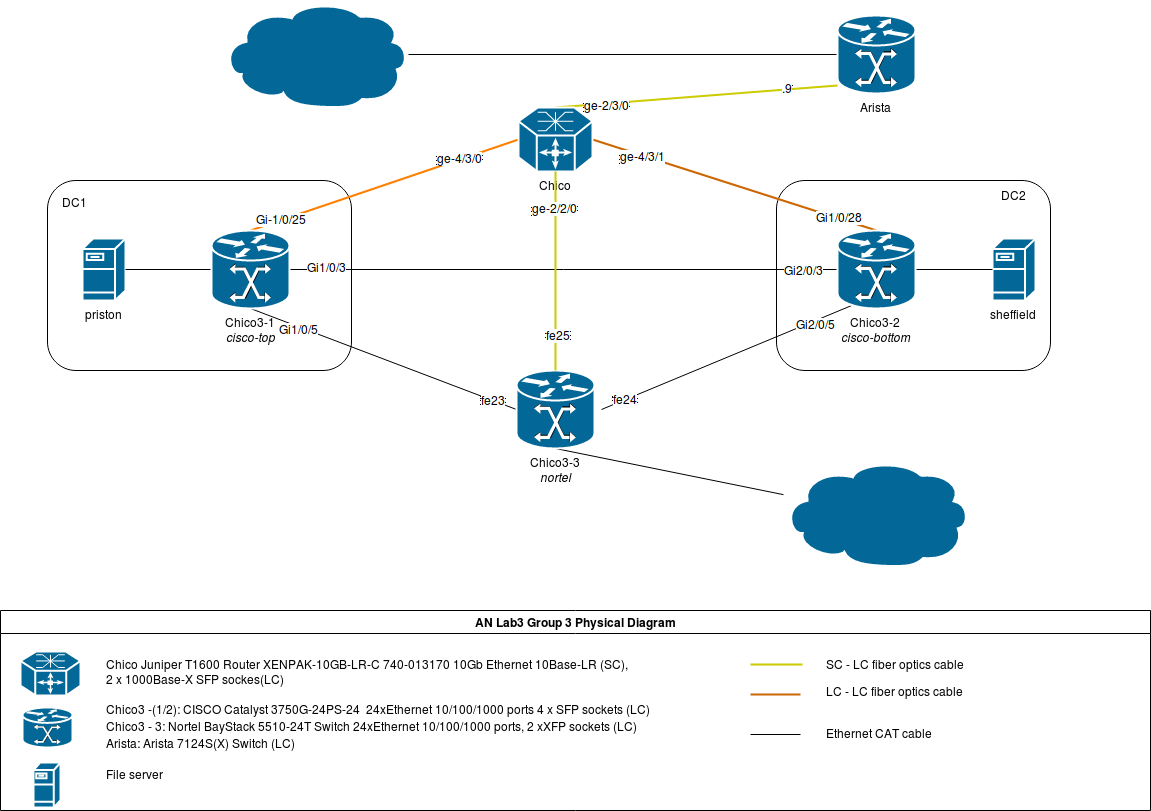
\includegraphics[width=\textwidth]{ANLab3Group3PhysicalDia.png}
\end{frame}

\begin{frame}{Design}{Network logical topology}
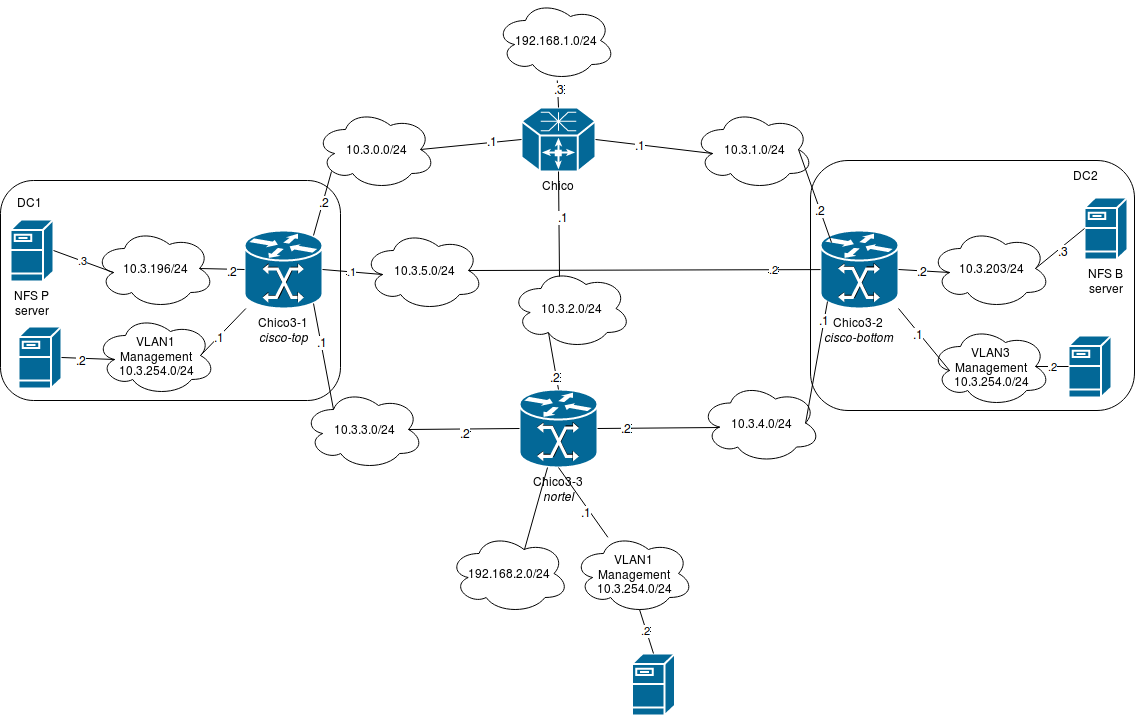
\includegraphics[width=\textwidth]{ANLab3Group3LogicalDia.png}
\end{frame}

\section{Implementation}
\begin{frame}{Implementation}{Challenges}
\begin{itemize}
    \item Not all SPF sockets of Cisco switches are operational.
    \item Nortel require a license for OSPF.
    \item Nortel supports only STP, no different refinements like Cisco.
    \item Nortel is bankrupt, so no support available.
\end{itemize}
\end{frame}

%\section{Exam}
%\begin{frame}{Exam}{NFS demonstration}
%Turn off NFS on one of the NFS servers and show file is still accessible.
%\end{frame}

%---------------------------------------------------------------------------


%%%%%%%%%%%%%%%%%
\section{Conclusion}
\begin{frame}{Conclusion}
\begin{block}{}
\begin{itemize}
\item	Proper inventorization might spare implementation time.
\item	Due to a proper standards implementation even different manufactured devices can communicate with each other.
\item   Fiber optics require some effort to setup it physically, but works similar to Ethernet. 
\item No auto-negotiation for optics provides extra limitations during design stage.
\item   Take into account that theory is not reality

\end{itemize}
\end{block}


\end{frame}

\begin{frame}[allowframebreaks]{Questions?}

THANK YOU!

\def\newblock{}
\bibliographystyle{unsrt}
\bibliography{mybib}
\end{frame}
\end{document} 
%---------------------------------------------------------------------------
